\documentclass[10.5pt, oneside]{article}
% \usepackage[margin=1in]{geometry}
\usepackage[left=0.80in,right=0.80in,top=0.8in,bottom=0.8in]{geometry}
\geometry{letterpaper}
\usepackage{booktabs}
\usepackage{hyperref}
\usepackage{enumitem}
\usepackage{float}
\usepackage{caption}
\usepackage{subcaption}
\usepackage[numbers]{natbib}
\usepackage{graphicx}
\usepackage{amssymb}
\usepackage{amsmath}
\usepackage{multirow}
\usepackage{array}
\usepackage{xcolor}

\title{OBELIX: the Warehouse Robot \\ \Large{CS780 Capstone Project}
}

\author{
    Aritra Ambudh Dutta  \\
    230191\\
   {\tt aritraad23@iitk.ac.in}\\
{Indian Institute of Technology Kanpur}
}

\date{}

\begin{document}

\maketitle

\begin{abstract}
This report explores reinforcement learning for the OBELIX warehouse robot, which must find, attach to, and push a grey box to the arena boundary in a Partially Observable Markov Decision Process (POMDP) with 18-bit binary sensors. Over four phases, majorly seven approaches were investigated---DQN, Dueling D3QN with GRU, Recurrent PPO, Discrete SAC, and hybrid heuristic-RL---employing potential-based reward shaping, curriculum learning, frame stacking, and prioritized experience replay. Sparse rewards and perceptual aliasing caused persistent circling failures across most methods. The best agent, \textbf{Recurrent PPO with LSTM}, scored $\textbf{-1447.55}$ on the Codabench final test phase.
\end{abstract}

\section{Competition Result}
\textbf{Codabench Username:} a\_230191 \\
\textbf{Final leaderboard rank (Test Phase):} 11 \\
\textbf{Leaderboard rank -- Level 1 (static):} 39 \\
\textbf{Leaderboard rank -- Level 2 (blinking):} 80 \\
\textbf{Leaderboard rank -- Level 3 (moving + blinking):} 48 \\

\textbf{Number of valid submissions made:}

\begin{table}[H]
\centering
\begin{tabular}{l c}
\toprule
\textbf{Phase} & \textbf{Submissions} \\
\midrule
Development -- Level 1 (Static) & 15 \\
Development -- Level 2 (Blinking) & 11 \\
Development -- Level 3 (Moving + Blinking) & 53 \\
Final Test Phase & 366 \\
\bottomrule
\end{tabular}
\caption{Number of valid submissions per phase.}
\end{table}

\section{Introduction and Problem Description}

The OBELIX project draws inspiration from the seminal 1991 work by Mahadevan and Connell \cite{mahadevan1992automatic}, which demonstrated one of the earliest applications of reinforcement learning on a physical robot for box-pushing tasks. Our task is to design an RL-based autonomous controller for a simulated mobile robot named OBELIX that must locate a grey box in an arena, attach to it, and push it to the arena boundary (success).

The environment presents a \textbf{Partially Observable Markov Decision Process (POMDP)} with the following characteristics:

\begin{itemize}[nosep]
    \item \textbf{Observations}: An 18-bit binary vector consisting of 8 near sonar sensors, 8 far sonar sensors, 1 infrared (IR) sensor for direct frontal detection, and 1 indicator showing whether the robot is stuck against a wall or boundary.
    \item \textbf{Actions}: 5 discrete actions -- rotate left 45\textdegree{} (L45), rotate left 22.5\textdegree{} (L22), move forward (FW), rotate right 22.5\textdegree{} (R22), and rotate right 45\textdegree{} (R45).
    \item \textbf{Rewards}: Sparse and one-time (per-episode) sensor rewards (+1 for side sensors, +2 for far forward, +3 for near forward, +5 for IR), a large box attachment bonus (+100), push penalty ($-1$/step while pushing), huge success bonus (+2000), wall collision penalty ($-200$), and idle penalty ($-1$/step with no sensor activated).
\end{itemize}

The task is evaluated across \textbf{three }difficulty levels of increasing complexity:

\begin{enumerate}[nosep]
    \item \textbf{Level 1: Static Box}: The box remains stationary. The robot navigates to it, attaches, and pushes to the boundary.
    \item \textbf{Level 2: Blinking Box}: The box randomly appears and disappears. The robot cannot attach when the box is invisible, but once attached, blinking stops.
    \item \textbf{Level 3: Moving + Blinking Box}: The box moves with constant velocity and also blinks. Movement stops once the robot attaches.
\end{enumerate}

Additionally, a \textbf{vertical wall with a small opening} may appear in any level, introducing navigation obstacles with a harsh $-200$ penalty for wall collisions. The evaluation uses hidden random seeds across 10 runs per difficulty level, making overfitting to specific configurations infeasible.

The core challenges are: (1) \textbf{perceptual aliasing}: Under partial observability, many world states map to identical observations (especially all-zeros when the box is out of range); (2) \textbf{sparse rewards}: randomly finding, attaching, and pushing the box is highly unlikely; and (3) \textbf{exploration-exploitation trade-off}: systematic exploration when no informative sensors are active, and efficient exploitation once sensor cues become available. The goal was to maximize \textbf{mean cumulative reward} across all levels with wall robustness.

\section{Methodology and Model Evolution}

My work evolved significantly across the four development phases, with each iteration informed by the failures and insights of prior attempts.

\subsection{Phase 1--2: Initial Exploration (Levels 1 and 2)}

I explored six baseline algorithms: \textbf{(a) Standard DQN} (18$\to$64$\to$64$\to$5 MLP, 1K--2K episodes): consistently converged to a degenerate circling policy (L22$\leftrightarrow$R22), scoring $\approx$$-1980$; \textbf{(b) Tabular Q-Learning} ($2^{18}$ = 262K states, up to 1M episodes): slow convergence due to enormous state space; \textbf{(c) A2C} (shared actor-critic, 5K episodes): marginally better exploration but still failed to find the box; \textbf{(d) Dueling DRQN} (GRU-based, 18$\to$64$\to$GRU(64)$\to$5, 4-frame stack): had memory capability but still circled; \textbf{(e) DRQN with Anti-Rotation Reward Shaping} ($-0.2$ anti-rotation penalty after sustained turn streaks, with an additional $-0.5$ penalty under prolonged same-observation turning; $+1.5$ FW bonus on zero sensors to discourage Rotation; 72-dim input through a 16-step GRU): theoritically best Phase 1--2 approach but still scored $-1980$ on Codabench; \textbf{(f) Dueling DDQN with Memory Augmentation} (22-dim input: 18 raw + visibility flag, steps-since-seen, sin/cos angle to box; 128-unit shared layers with dueling heads): could have helped when the box was blinking, but still could not solve the main challenge of reliably finding the box.

\subsubsection{Root Cause Analysis}

After Phase 1--2, I identified four reasons for the persistent circling behavior: (1) \textbf{Perceptual aliasing}: many world states map to identical observations, especially the all-zeros case; (2) \textbf{Deceptive rewards}: Positive rewards are sparse and hard to reach, while random forward exploration often causes immediate penalties (e.g., \textit{collisions/idle loss}), so the agent finds repetitive turning safer than risky movement toward true task completion; (3) \textbf{Exploration failure}: $\epsilon$-greedy cannot reliably find the box; (4) \textbf{Shaping distortion}: aggressive bonuses caused optimization for shaped rather than true rewards.

\subsection{Phase 3: Structured Approaches (Level 3)}

Based on the analysis, I developed four structured approaches:

\textbf{Approach 1 -- Recurrent PPO (RPPO)} \cite{schulman2017proximal}: LSTM-based actor-critic (77-dim input: 4-frame stack + one-hot prev-action, 128-unit LSTM). Curriculum learning over 5 phases (spawn distance: 20px $\to$ random) with 7-component dense reward shaping. Performed well in training but poorly on Codabench's random spawns ($-1500$ to $-4000$).

\textbf{Approach 2 -- Dueling D3QN + GRU + PER} \cite{wang2016dueling, van2016deep, schaul2015prioritized}: 128-unit GRU with Prioritized Experience Replay (PER) ($\alpha\!=\!0.6$, $\beta$: 0.4$\to$1.0 via SumTree) and 3-step returns. Same input/curriculum as Approach 1. Best single-episode score in Phase 3 ($-1515$) but inconsistent.

\textbf{Approach 3 -- Discrete SAC} \cite{haarnoja2018soft}: Entropy-regularized $J(\pi) = \mathbb{E}[Q(s,a) - \alpha \log \pi(a|s)]$ with twin GRU-based Q-networks and auto-tuned temperature ($\alpha$), to encourage exploration and reduce premature collapse to circling policies. In our Phase 3 runs, it did not converge within the available training budget.

\textbf{Approach 4 -- Hybrid Heuristic + DQN}: Mode-switch hybrid controller with hand-crafted search/stuck-escape heuristics and a small DQN (77$\to$64$\to$64$\to$5) for sensor-active approach/push decisions (with heuristic--NN blending). Practical for reducing random wandering, but still brittle with wall obstacles.


\subsection{Phase 4: Final Approaches (Test Phase)}

Phase 3 established the core design logic, but its results were \textbf{limited by both compute and tuning}: the runs were configured with max\_steps $=1000$, intended 8K--10K episodes, and relatively large replay settings, yet most experiments had to stop early (typically around \(\sim\)2K episodes) due to limited compute. In addition, these settings were not always well matched to the task (for \textit{long-horizon sparse-reward exploration}), so Phase 3 outcomes should be interpreted as \textbf{\textit{under-trained or suboptimally tuned}} rather than definitive failures of the underlying ideas.

In Phase 4, I kept the previous Phase 3 approaches for continuity and fair re-checking, but introduced \textbf{three new methods} (Approaches 5--7), including \textbf{no-curriculum variants} (Approaches 5 and 6) motivated directly by the Phase 3 shortcomings. Thus, the final iteration covered \textbf{7 total approaches} (4 retained + 3 new). The Phase 4 setups used \textbf{tuned hyperparameters with sufficient compute} (typically 10K--15K episodes, max\_steps $=2000$, replay sizes about 50K--75K), which improved stability and yielded stronger Codabench results.

The practical reason these changes helped is that \textbf{longer episodes with higher max\_steps} exposed the full search$\rightarrow$approach$\rightarrow$push trajectory more often, while \textbf{moderate replay sizes} reduced the dominance of stale early transitions from weak policies. Together, this made \textit{training updates less noisy under sparse rewards} and made optimization less noisy than the short-horizon, over-large-buffer Phase 3 setting.\\
\noindent This led to three refined approaches:


\textbf{Approach 5 -- Simple DDQN without Curriculum}: I used a 3-layer MLP (two hidden layers: $77 \to 128 \to 128 \to 5$) Double DQN with \textbf{no curriculum learning} and \textbf{minimal reward shaping} (only anti-circling: $-3.0$ for 6+ consecutive turns, and anti-stuck: $-10.0$). The key innovation was a \textbf{heuristic fallback/search policy} at inference: when all sensors are zero, instead of relying on NN outputs, the agent follows a rule-based ``\textit{lawnmower}'' pattern (15 forward steps, then a 90\textdegree{} turn via two 45\textdegree{} turns, alternating direction). Training used mixed difficulty sampling per episode (0/2/3), with wall obstacles always enabled, for 15,000 episodes.

\textbf{Approach 6 -- D3QN v2 with GRU, No Curriculum}: Similar philosophy of minimal intervention applied to the recurrent architecture. Dueling D3QN with 128-unit GRU, 77-dim input, 16-step sequences. No curriculum, minimal shaping. The GRU hidden state was reset after 5 consecutive zero-observations to prevent saturation. Trained for 12,000 episodes across mixed difficulties with $wall\_obstacles=True$ always.

% \textbf{Approach 7 -- Refined D3QN with PBRS}: My most principled approach used Potential-Based Reward Shaping (PBRS) \cite{ng1999policy}, which is theoretically guaranteed to preserve optimal policies. Three shaping components were used:
% \begin{align}
%     \Phi_{\text{approach}}(s) &= -\frac{d(\text{robot}, \text{box})}{d_{\text{max}}} \\
%     \Phi_{\text{heading}}(s) &= \cos(\theta_{\text{facing}} - \theta_{\text{to\_box}}) \quad \text{(pre-attachment only)} \\
%     \Phi_{\text{push}}(s) &= -\frac{d(\text{box}, \text{nearest\_wall})}{d_{\text{max}}} \quad \text{(post-attachment only)}
% \end{align}
% The shaped reward at each step was $F(s, s') = \gamma \Phi(s') - \Phi(s)$ with a scaling factor of 10.0. The architecture used a larger Dueling DQN (256$\to$128 shared encoder) with 6-frame stacking (108-dim input), PER ($\alpha=0.6$), and 3-step returns. Curriculum was reintroduced but more conservatively (4 phases over 8000 episodes). Trained with max\_steps=2000.
\textbf{Approach 7 -- Refined D3QN with PBRS}: My last approach used Potential-Based Reward Shaping (PBRS) \cite{ng1999policy}, which is theoretically guaranteed to preserve optimal policies. Three shaping components were used:
\begin{align}
    \Phi_{\text{approach}}(s) &= -\frac{d(\text{robot},\text{box})}{d_{\text{max}}} \\
    \Phi_{\text{heading}}(s) &= \cos(\theta_{\text{facing}} - \theta_{\text{to\_box}}) \quad \text{(pre-attachment only)} \\
    \Phi_{\text{push}}(s) &= -\frac{d(\text{box, nearest\_wall})}{d_{\text{max}}} \quad \text{(post-attachment only)}
\end{align}
The shaped reward at each step followed $F(s, s') = \gamma \Phi(s') - \Phi(s)$ with a global shaping scale of 10.0; in implementation, heading and push terms were additionally weighted by 0.5 and 2.0 respectively. The architecture used a larger Dueling Double DQN (shared encoder: $108 \to 256 \to 128$ via 6-frame stacking), with PER ($\alpha=0.6$) and 3-step returns. Curriculum was reintroduced conservatively in four phases (no-wall warm-up $\to$ walls $\to$ blinking $\to$ full 0/2/3 mix over 8,000 episodes), and training used \texttt{max\_steps}=2000.
\subsection{Detailed Description of Best Models}

\subsubsection{Approach 1: Recurrent PPO with LSTM (Best Score: $-1447.55$)}

\begin{itemize}[nosep]
    \item \textbf{Algorithm}: Proximal Policy Optimization (PPO) with LSTM-based recurrent actor-critic
    \item \textbf{Architecture}: Linear(77$\to$128) $\to$ ReLU $\to$ LSTM(128$\to$128) $\to$ Actor head (128$\to$5) + Critic head (128$\to$1)
    \item \textbf{State representation}: 4-frame stack (72 dims) + previous action one-hot (5 dims) = 77 dims
    \item \textbf{Training}: Curriculum learning (spawn near box early, random later), dense reward shaping (sensor proximity, IR alignment, anti-circling), GAE ($\lambda\!=\!0.95$), entropy regularization ($\beta\!=\!0.02$), PPO clipping ($\epsilon\!=\!0.2$)
    \item \textbf{Inference}: Greedy policy (argmax on actor logits). No heuristic fallback --- the LSTM's memory enables learned temporal strategies for the search phase.
\end{itemize}

\subsubsection{Approach 7: D3QN + PBRS (Best Score: $-1540.74$)}

\begin{itemize}[nosep]
    \item \textbf{Algorithm}: Dueling Double DQN with PER and n-step returns
    \item \textbf{Architecture}: Dueling MLP (108$\to$256$\to$128, then split into value head 128$\to$64$\to$1 and advantage head 128$\to$64$\to$5). $Q(s,a) = V(s) + A(s,a) - \text{mean}(A)$
    \item \textbf{State representation}: 6-frame stack (108 dims)
    \item \textbf{Exploration}: Forward-biased $\epsilon$-greedy with slow decay over 200K steps
    \item \textbf{Reward shaping}: 3-component PBRS (approach, heading, push) with scale 10.0 (heading ×0.5, push ×2.0)
    \item \textbf{Curriculum}: 4-phase progressive difficulty introduction
\end{itemize}

\section{Experiments and Implementation Details}

\subsection{Training Setup}

All experiments were conducted on a CPU-based environment (as required by the submission constraints) with Python 3 and PyTorch. All inference codes were designed to run on CPU with \texttt{map\_location=``cpu''}.

\subsection{Hyperparameter Summary}

\begin{table}[H]
    \centering
    \small
    \begin{tabular}{l c c c c c c c}
    \toprule
    \textbf{Parameter} & \textbf{Approach 1} & \textbf{Approach 2} & \textbf{Approach 3} & \textbf{Approach 4} & \textbf{Approach 5} & \textbf{Approach 6} & \textbf{Approach 7} \\
    \midrule
    Learning rate & 3e-4 & 1e-4 & 3e-4 & 2e-4 & 2e-4 & 1e-4 & 1e-4 \\
    $\gamma$ & 0.99 & 0.99 & 0.99 & 0.99 & 0.99 & 0.99 & 0.99 \\
    Batch size & -- & 64 & 128 & 64 & 64 & 64 & 64 \\
    Buffer size & -- & 75K & 75K & 50K & 75K & 75K & 50K \\
    $\epsilon$ decay & -- & 300K & -- & 100K & 500K & 500K & 200K \\
    Target update & -- & 1K & Soft ($\tau$=0.005) & 1K & 2K & 2K & 2K \\
    Episodes & 8K & 8K & 8K & 5K & 15K & 12K & 8K \\
    Max steps & 1K & 1K & 1K & 1K & 1K & 1K & 2K \\
    Input dim & 77 & 77 & 77 & 77 & 77 & 77 & 108 \\
    Frame stack & 4 & 4 & 4 & 4 & 4 & 4 & 6 \\
    Prev. action & Yes & Yes & Yes & Yes & Yes & Yes & No \\
    Recurrence & LSTM & GRU & GRU & No & No & GRU & No \\
    Curriculum & Yes & Yes & Yes & Yes & No & No & Yes \\
    PER & No & Yes & No & No & No & No & Yes \\
    n-step & -- & 3 & 1 & 1 & 1 & 1 & 3 \\
    \bottomrule
    \end{tabular}
    \caption{Hyperparameter comparison across Approaches 1--7 (in order). ``--'' indicates not applicable.}
    \label{tab:hyperparams}
    \end{table}


\subsection{Multi-Difficulty Training}

For the \textbf{no-curriculum approaches} (Approaches 5 and 6), this weighted multi-difficulty sampling was used from the very beginning of training. In contrast, the \textbf{curriculum-based approaches} (Approaches 1--4 and 7) used staged progression (easier settings first, then harder conditions such as walls/blinking/full mixed difficulty), with Approach 7 ending in the same mixed 0/2/3 setting for final robustness.

\subsection{Local Evaluation}


To reduce overfitting to specific seeds, local evaluation was performed with multiple random seeds per difficulty level, following the Codabench evaluation protocol. We used our custom \texttt{rank\_checkpoints\_codabench.py} script to automate checkpoint scoring and comparison.

\section{Results}

\subsection{Codabench Test Phase Results}

\begin{table}[H]
\centering
\small
\begin{tabular}{c l l r r}
\toprule
\textbf{\#} & \textbf{Method} & \textbf{Best Checkpoint} & \textbf{Best Score} & \textbf{Worst Score} \\
\midrule
1 & Recurrent PPO (LSTM) & ep7200 & \textbf{$-1447.55$} & $-387621$ \\
7 & Refined D3QN + PBRS & ep05200 & $-1540.74$ & $-265222$ \\
3 & Discrete SAC (GRU) & ep2000 & $-1655.64$ & $-381539$ \\
6 & D3QN v2, No Curriculum & D3QN\_FINAL\_V1 & $-9435.41$ & $-326035$ \\
2 & D3QN + GRU + PER & ep4000 & $-25715.40$ & $-378919$ \\
5 & Simple DDQN + Heuristic & ep500 & $-156899.23$ & $-318887$ \\
\bottomrule
\end{tabular}
\caption{Best Codabench score per approach on the final test phase (sorted by best score, higher is better). Scores are mean cumulative reward across 3 difficulty levels $\times$ 10 runs, with wall obstacles. Approach 4 (Hybrid Heuristic) was not submitted to the final phase as it performed immensely bad on \textit{Local Evaluation}.}
\label{tab:results}
\end{table}

\subsection{Training Curves (Approach 7 -- Refined D3QN with PBRS)}

\begin{figure}[H]
\centering
\begin{subfigure}[b]{0.48\textwidth}
    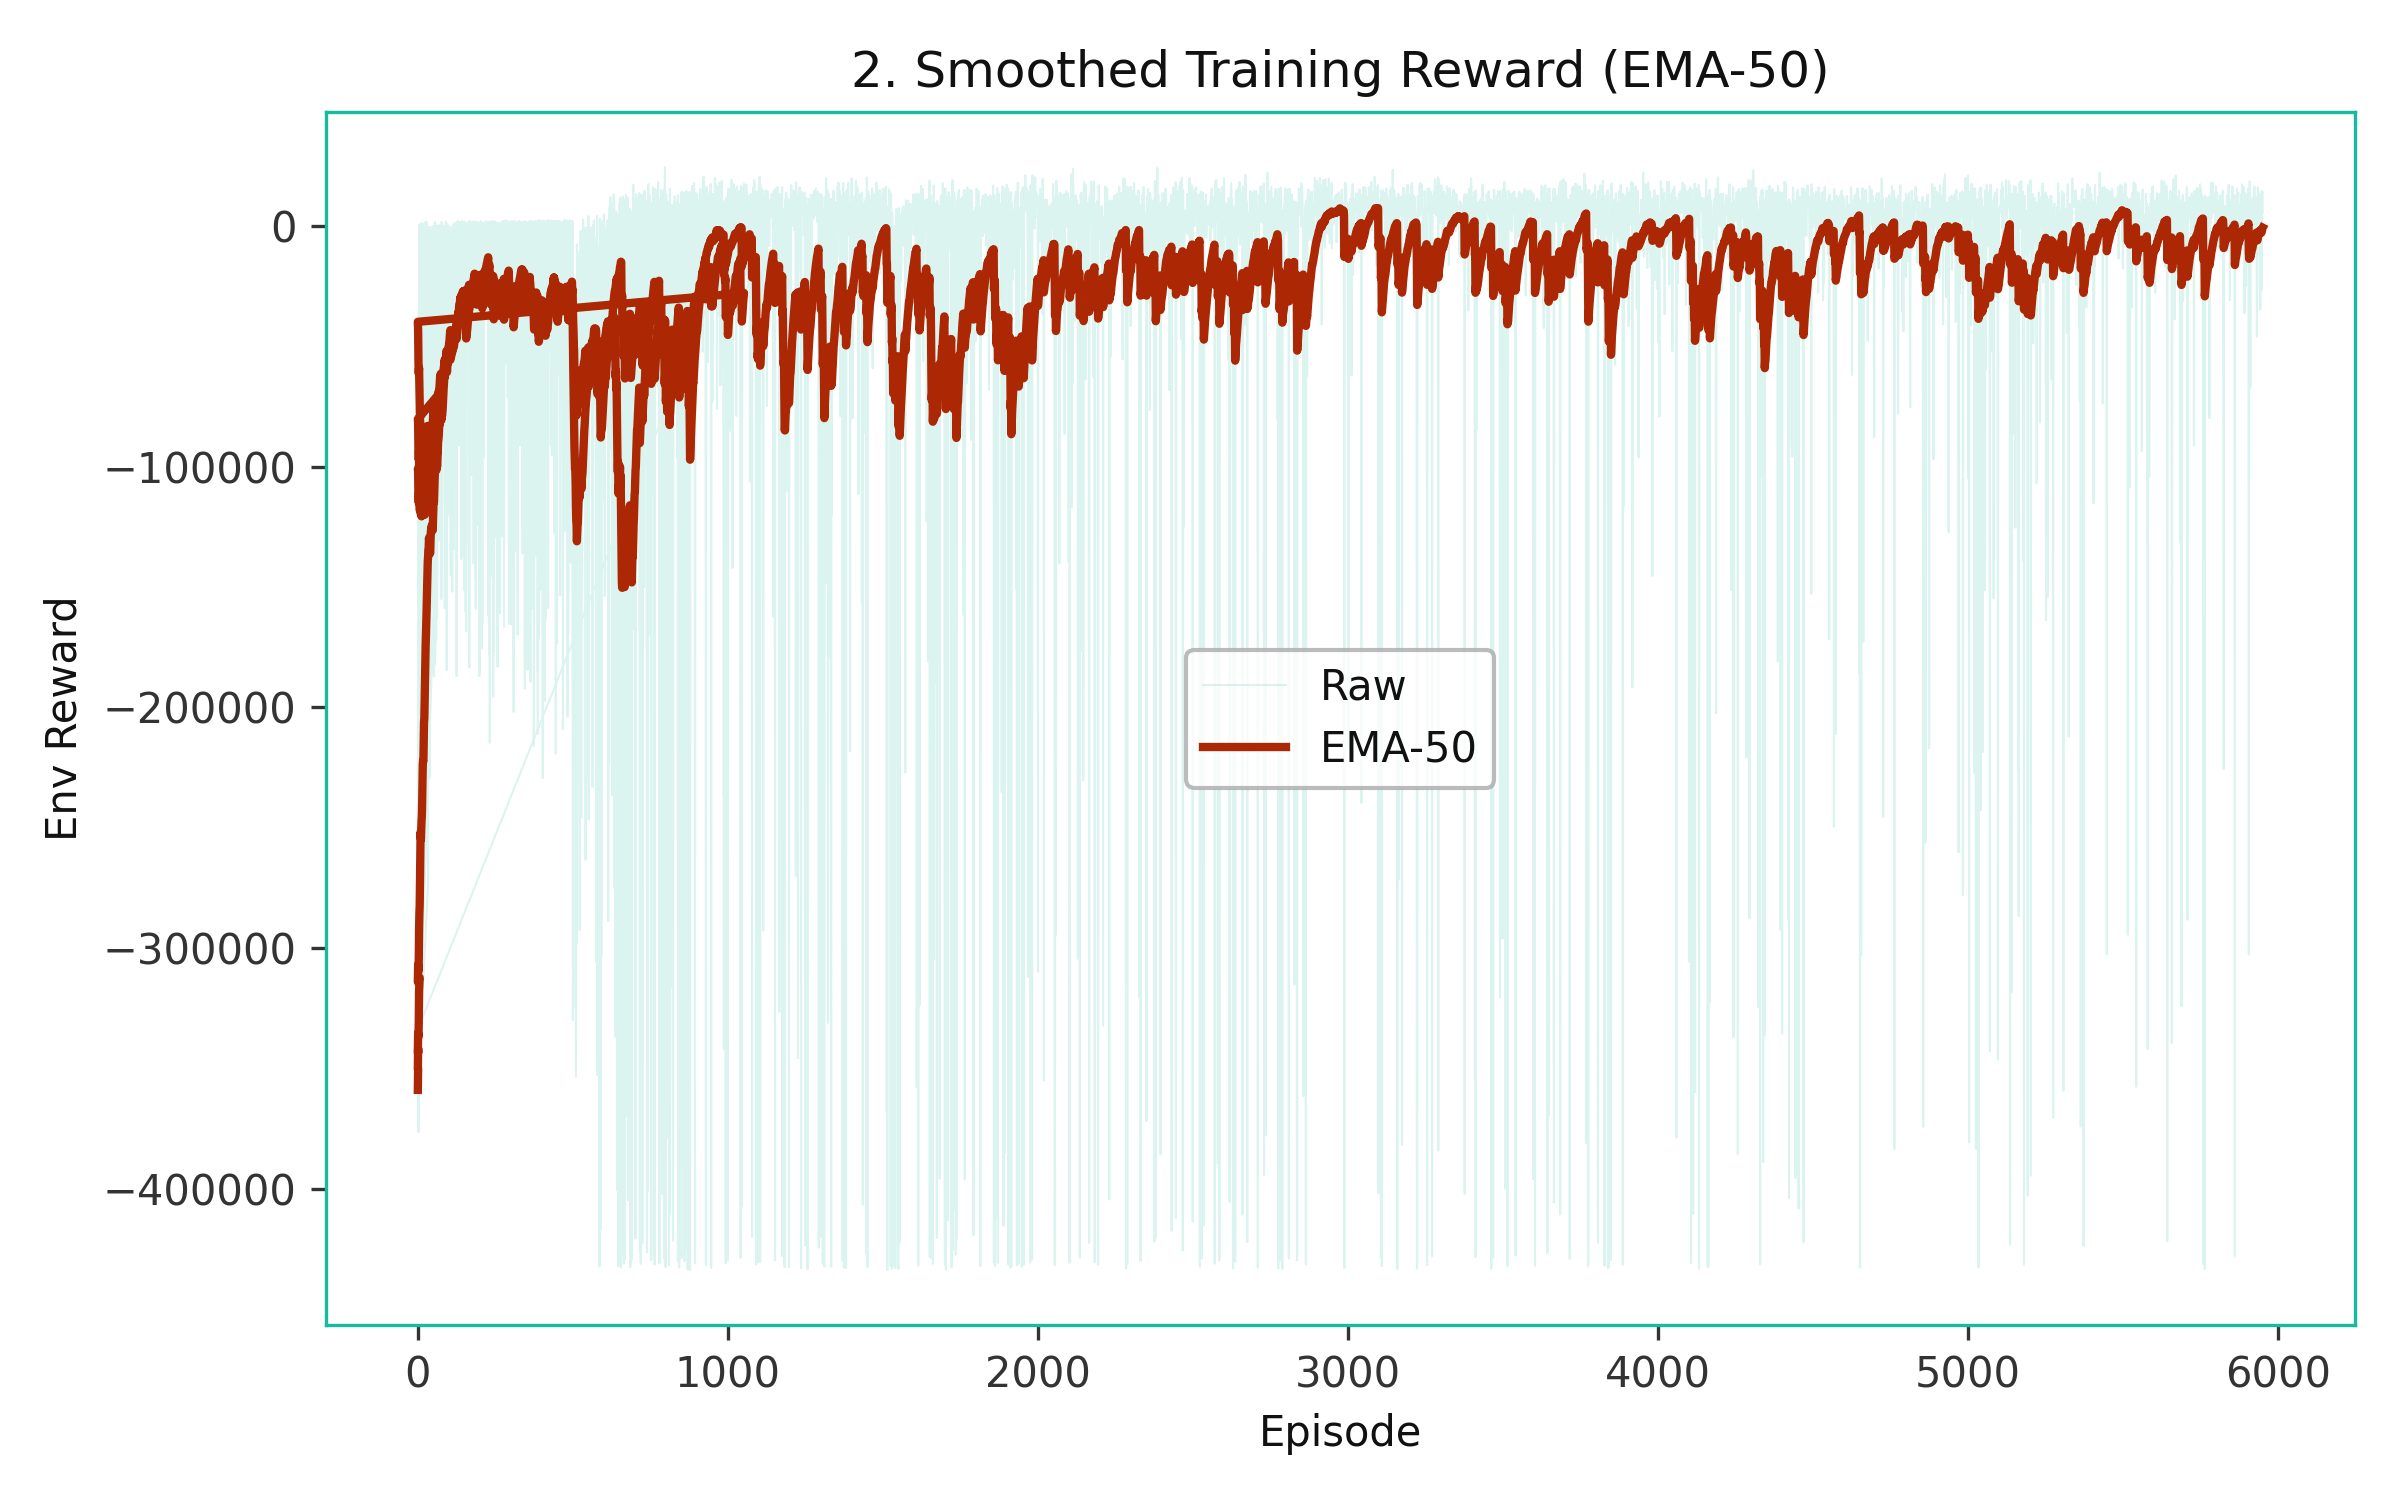
\includegraphics[width=\textwidth]{02_smoothed_reward.png}
    \caption{Smoothed training reward (EMA-50). Reward improves sharply after curriculum Phase 1, then stabilizes with high variance.}
    \label{fig:reward}
\end{subfigure}
\hfill
\begin{subfigure}[b]{0.48\textwidth}
    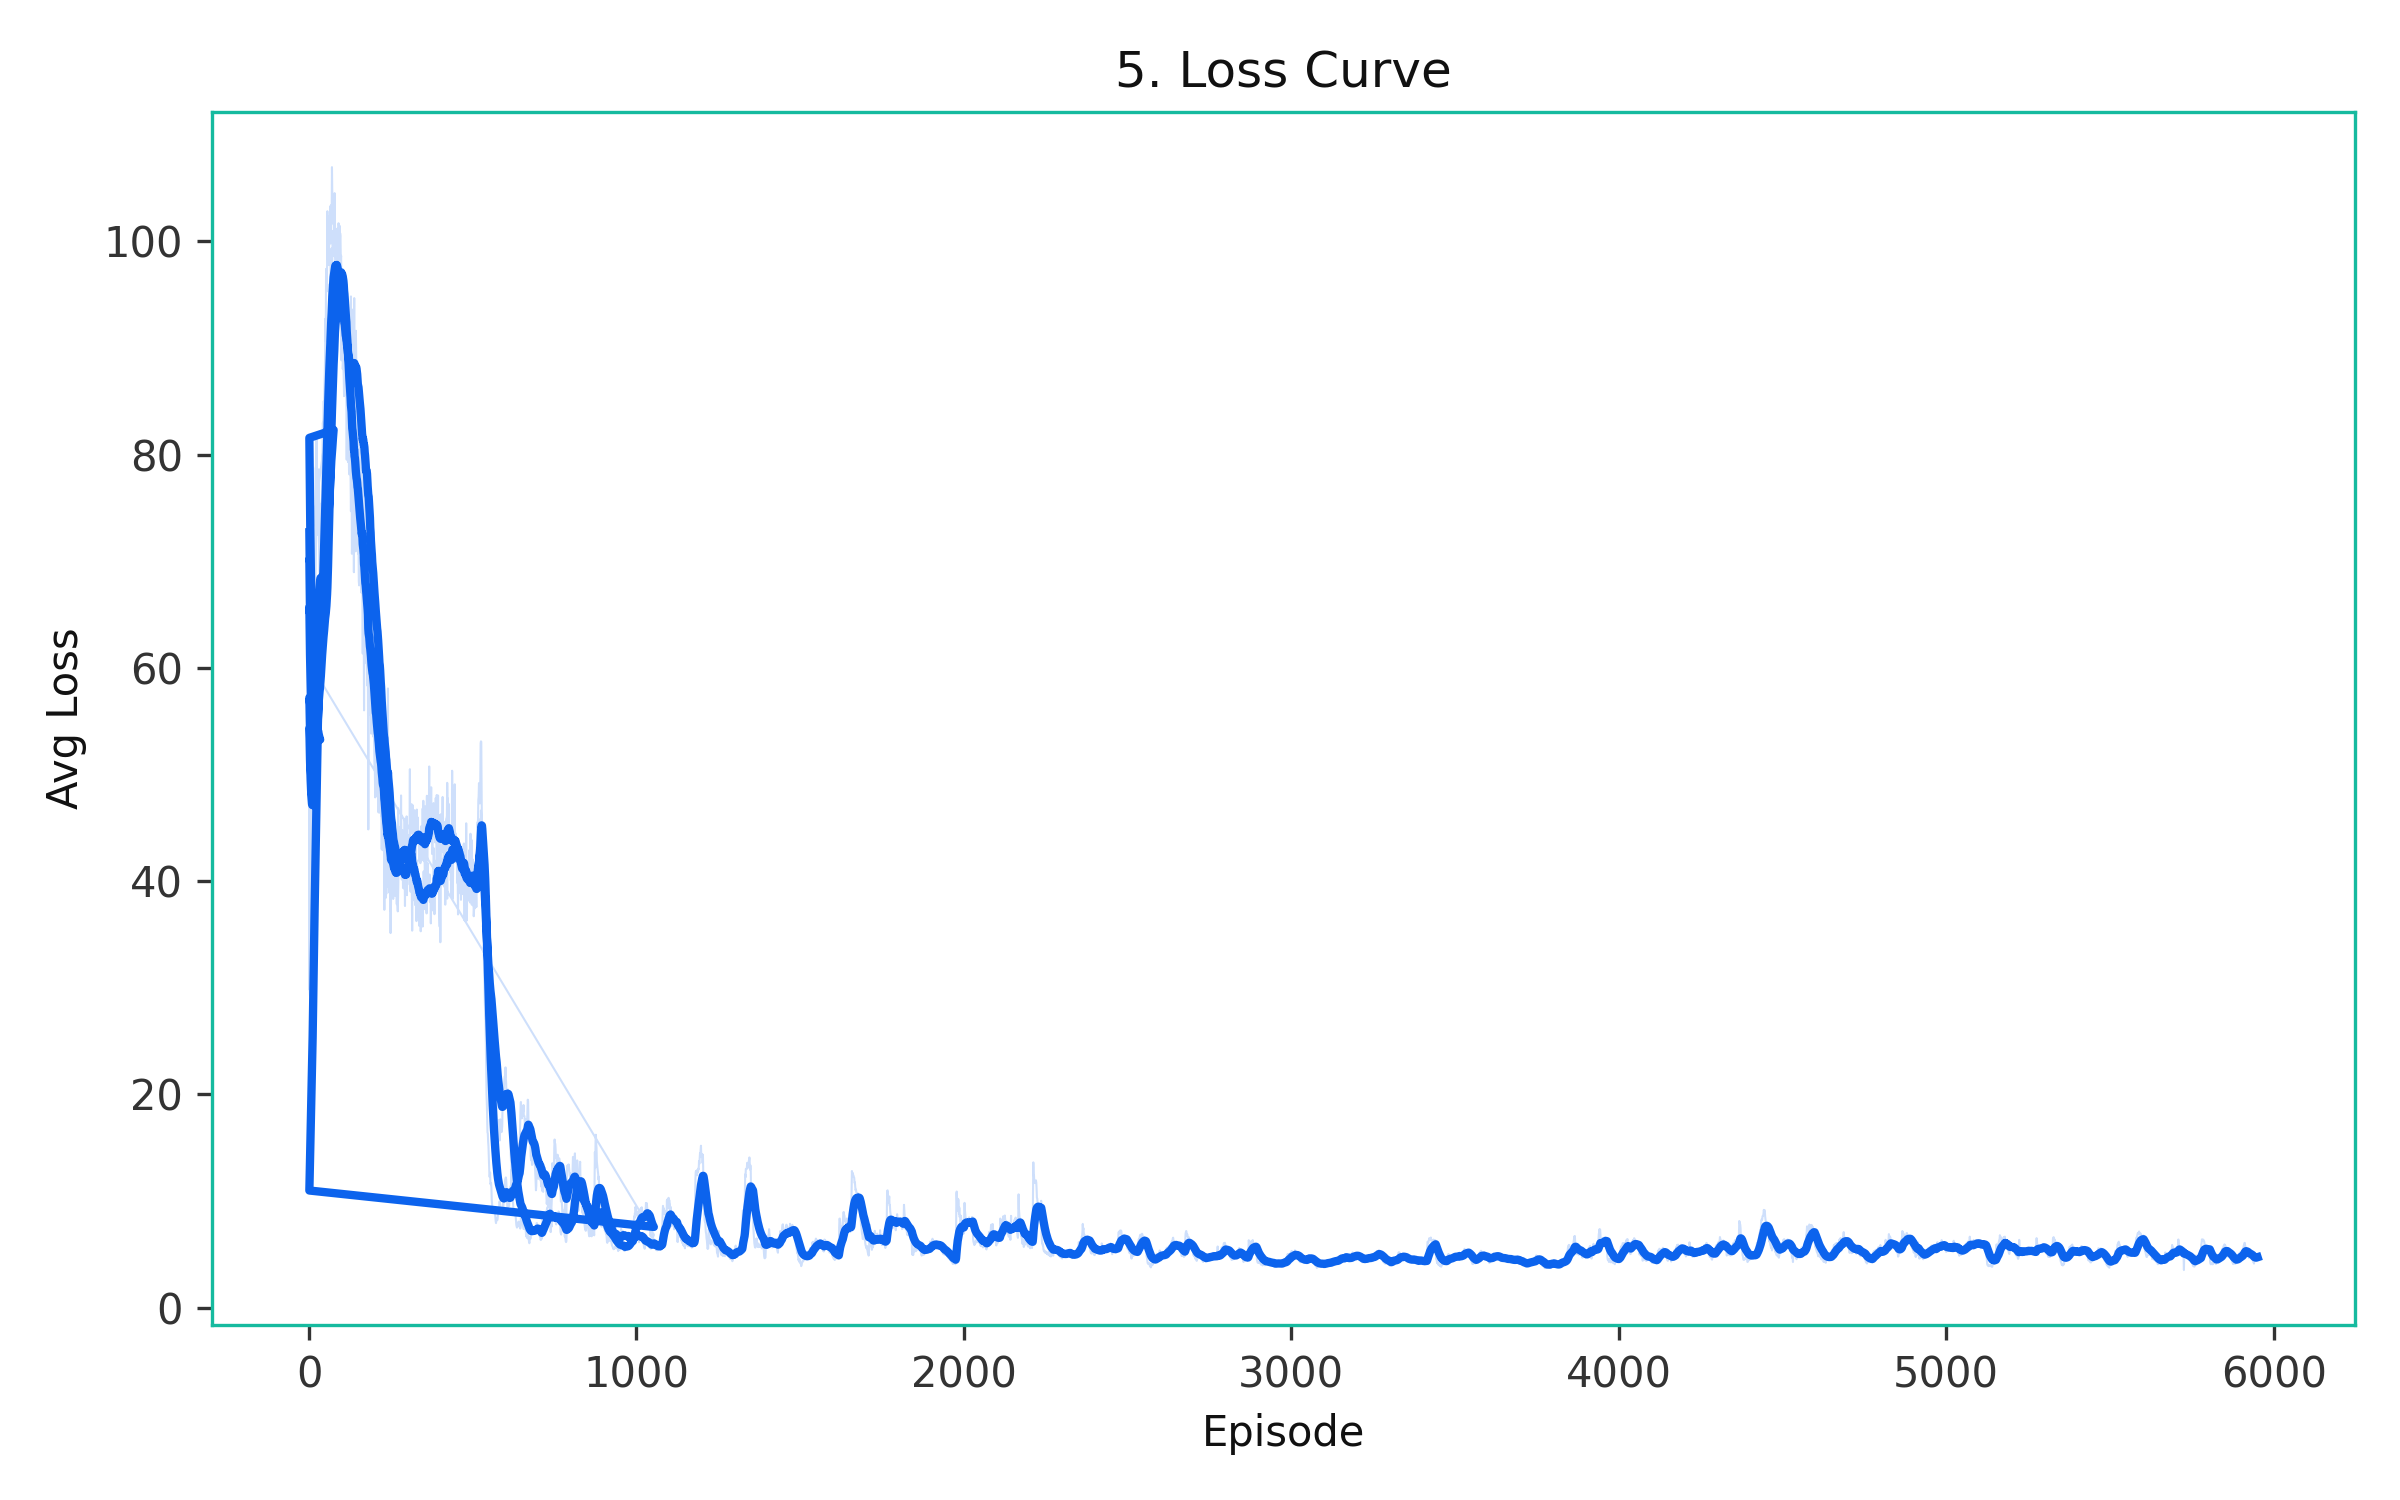
\includegraphics[width=\textwidth]{05_loss_curve.png}
    \caption{TD loss curve. Loss spikes during early episodes due to large reward magnitudes, then converges to a low stable value by episode 2000.}
    \label{fig:loss}
\end{subfigure}

\vspace{0.3cm}

\begin{subfigure}[b]{0.48\textwidth}
    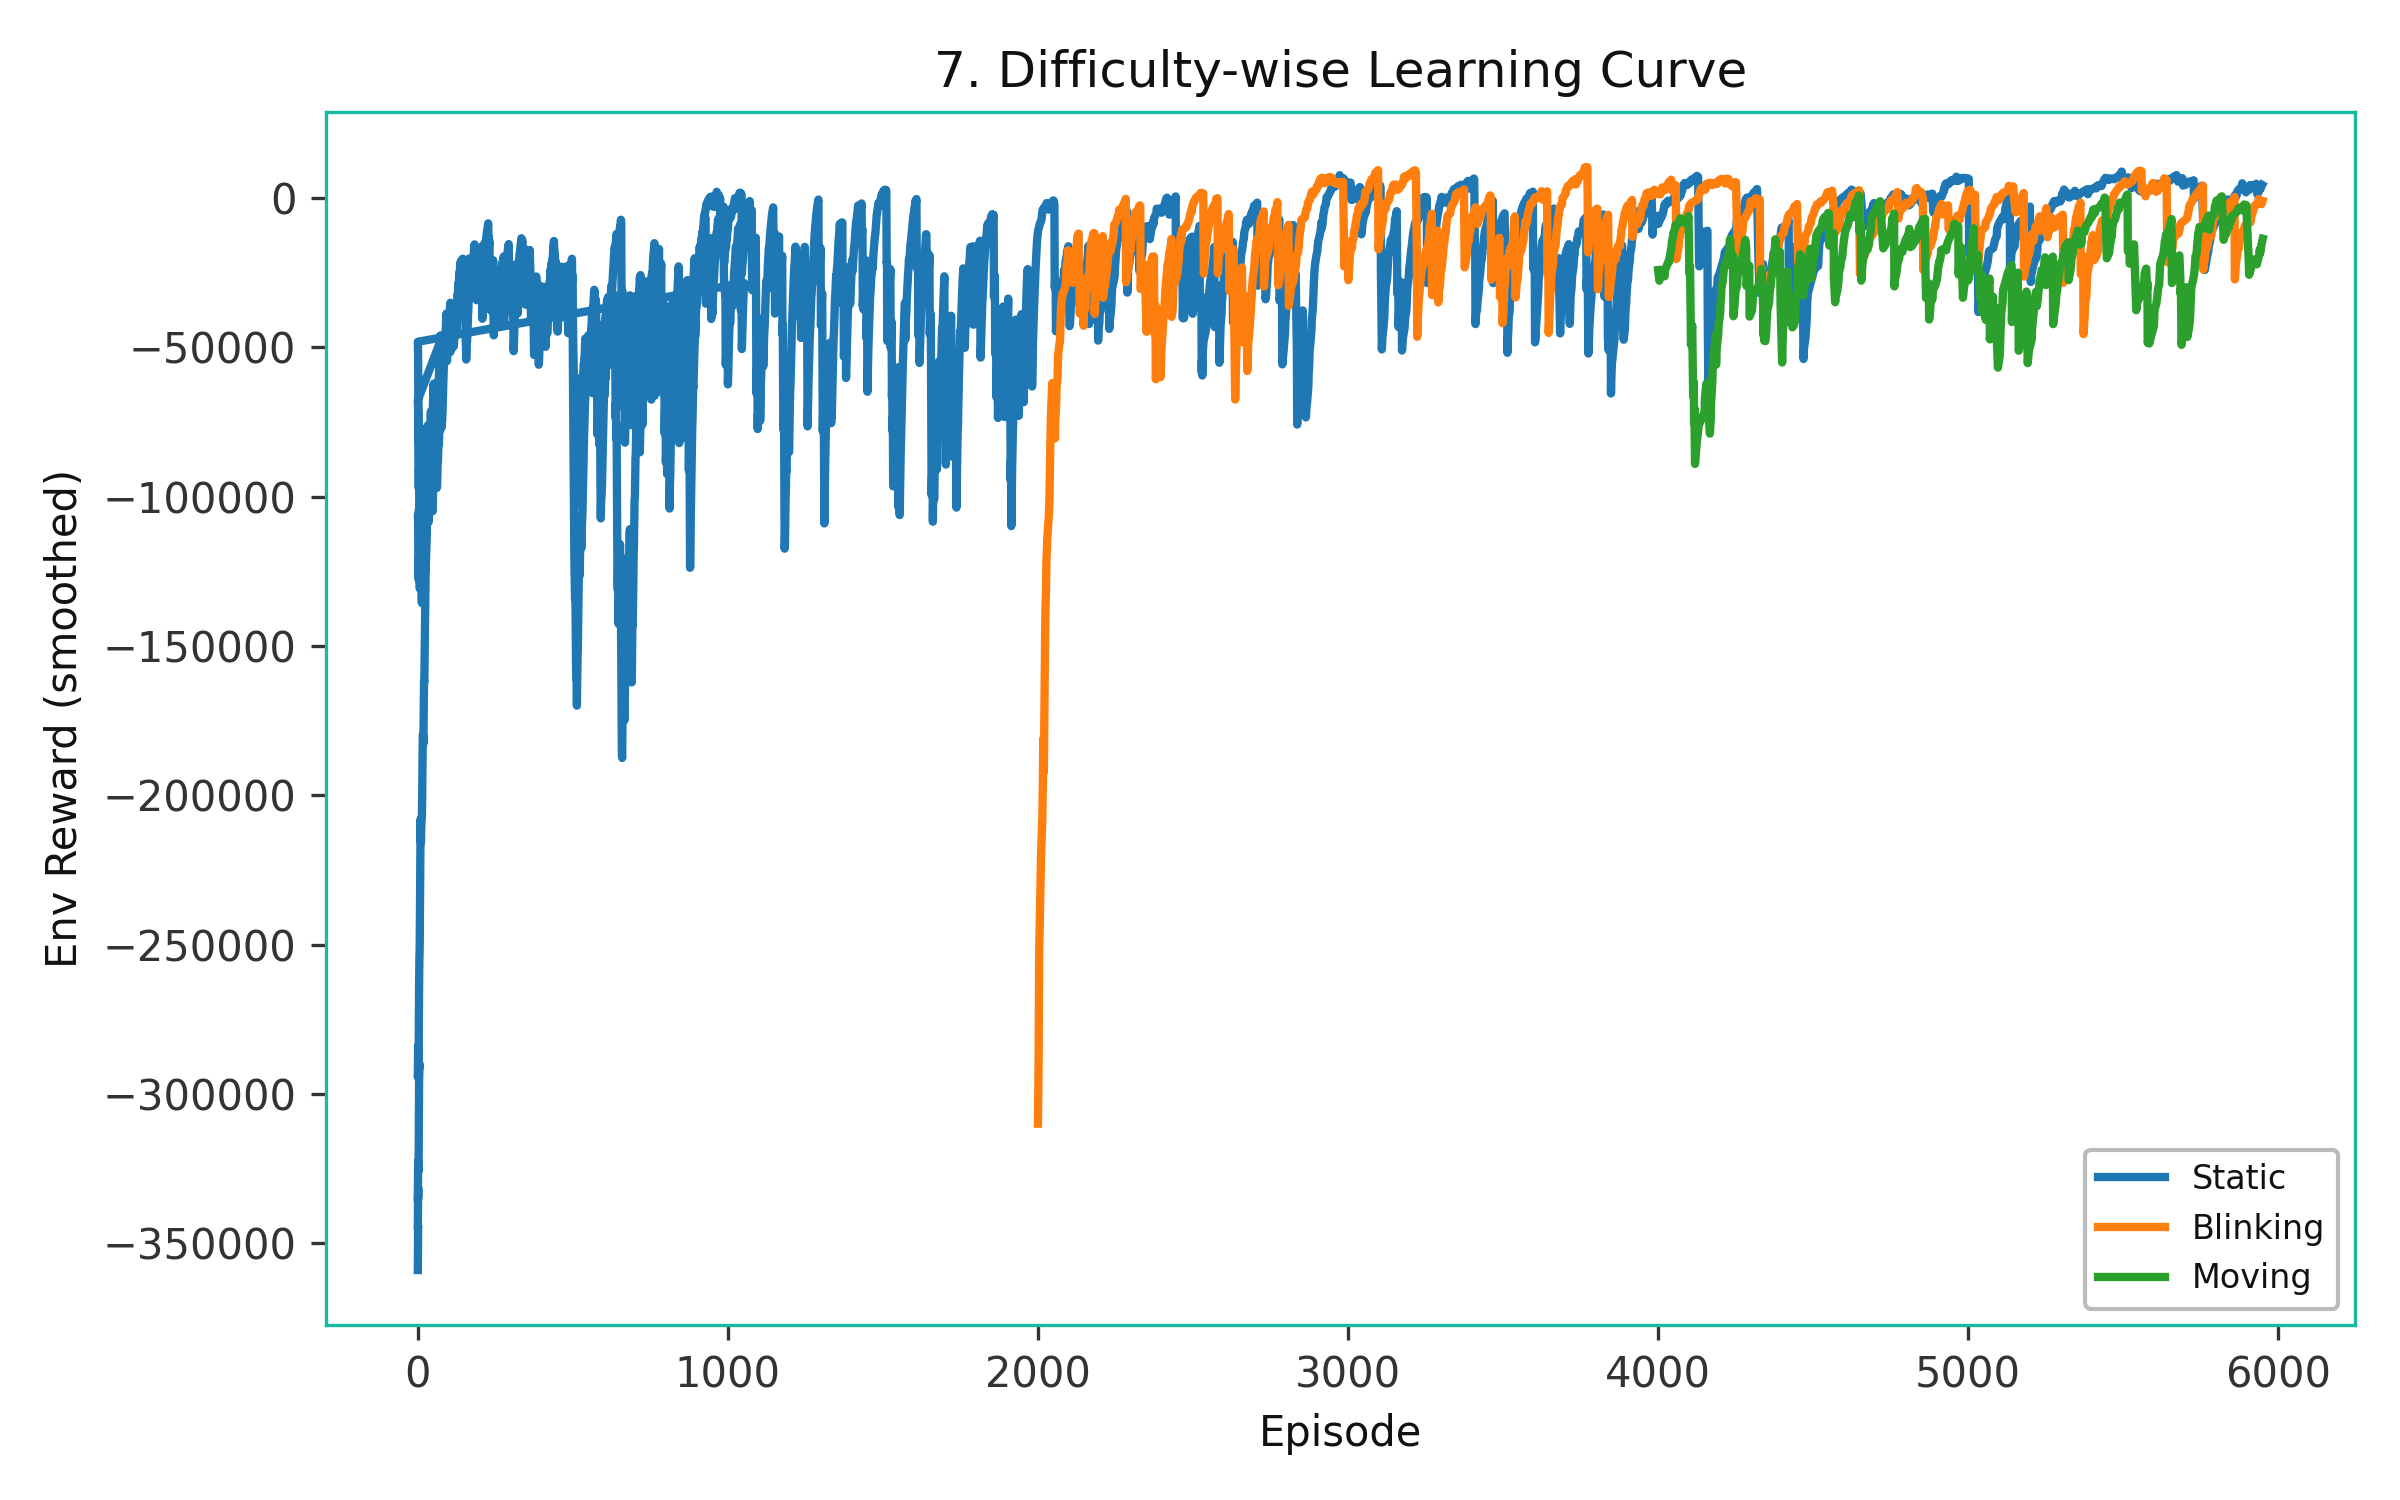
\includegraphics[width=\textwidth]{07_difficulty_learning.png}
    \caption{Per-difficulty learning curves. Static (Level 0) learns fastest; blinking and moving levels introduced later via curriculum show slower improvement.}
    \label{fig:difficulty}
\end{subfigure}
\hfill
\begin{subfigure}[b]{0.48\textwidth}
    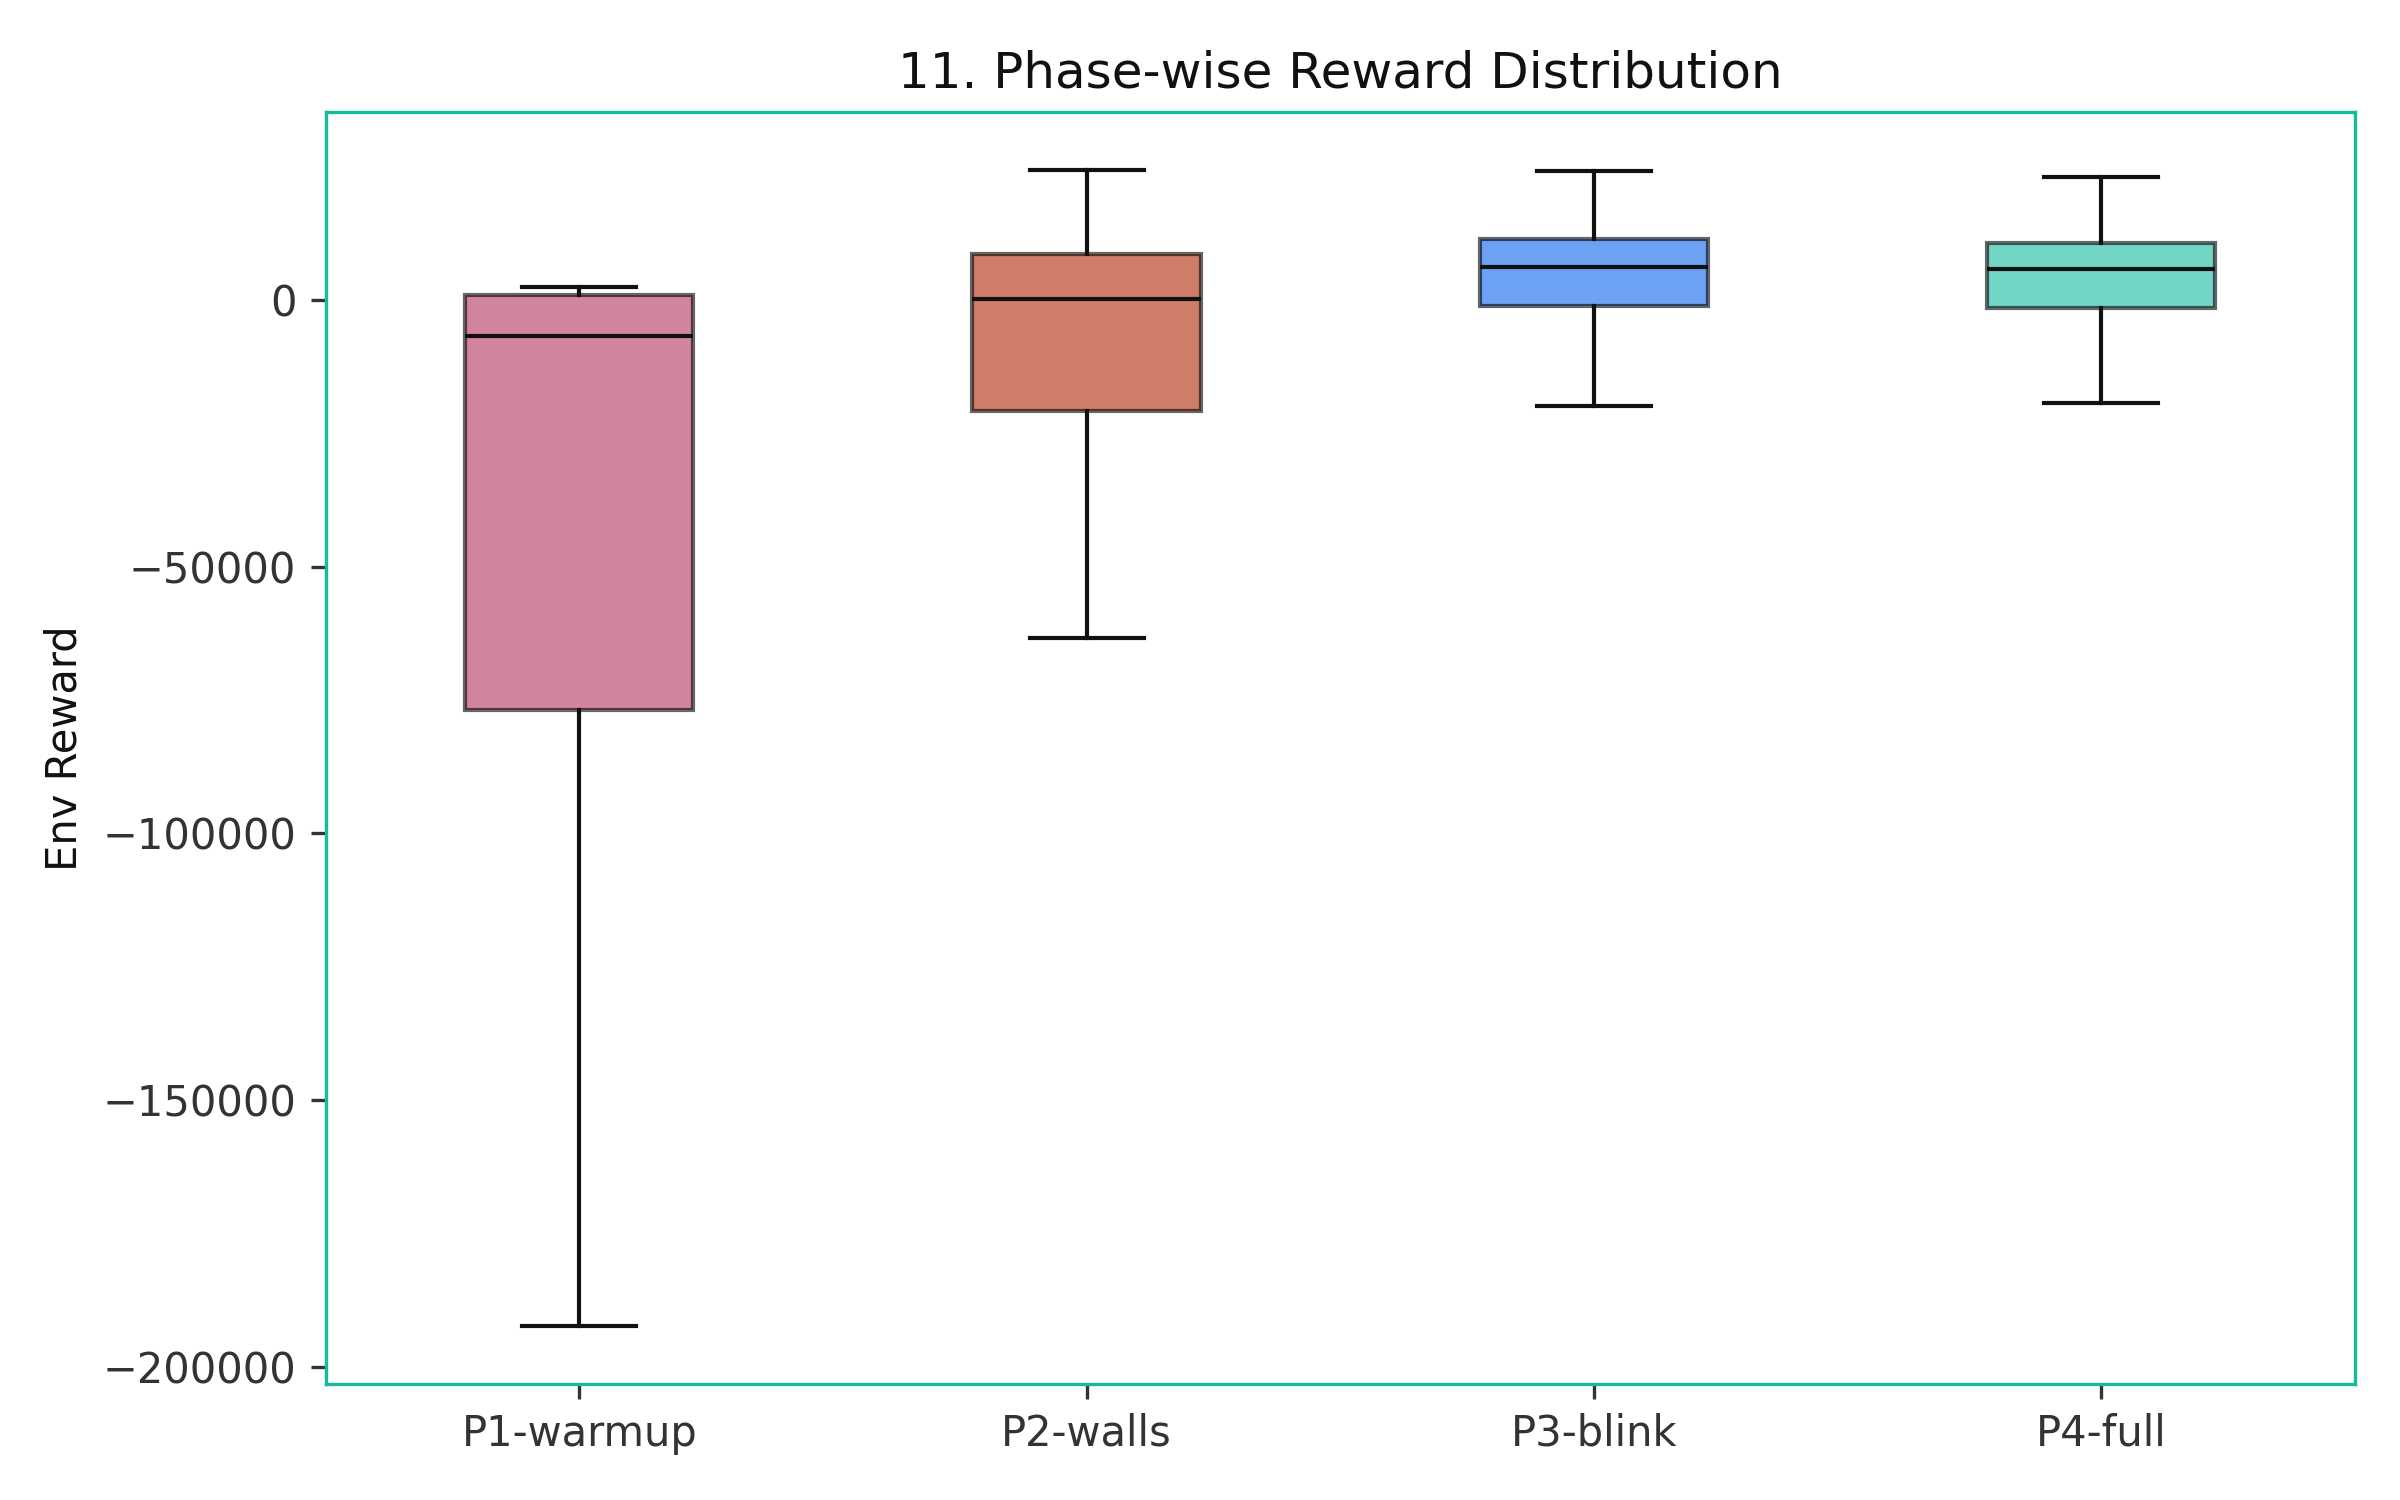
\includegraphics[width=\textwidth]{11_phase_rewards.png}
    \caption{Reward distribution per curriculum phase. Variance decreases and median reward improves across phases, indicating progressive learning.}
    \label{fig:phases}
\end{subfigure}
\caption{Training diagnostics for Approach 7 (Refined D3QN with PBRS, 6000 episodes). All plots use true environment reward (not shaped reward).}
\label{fig:training}
\end{figure}

\subsection{Codabench Score Analysis}

\begin{figure}[H]
\centering
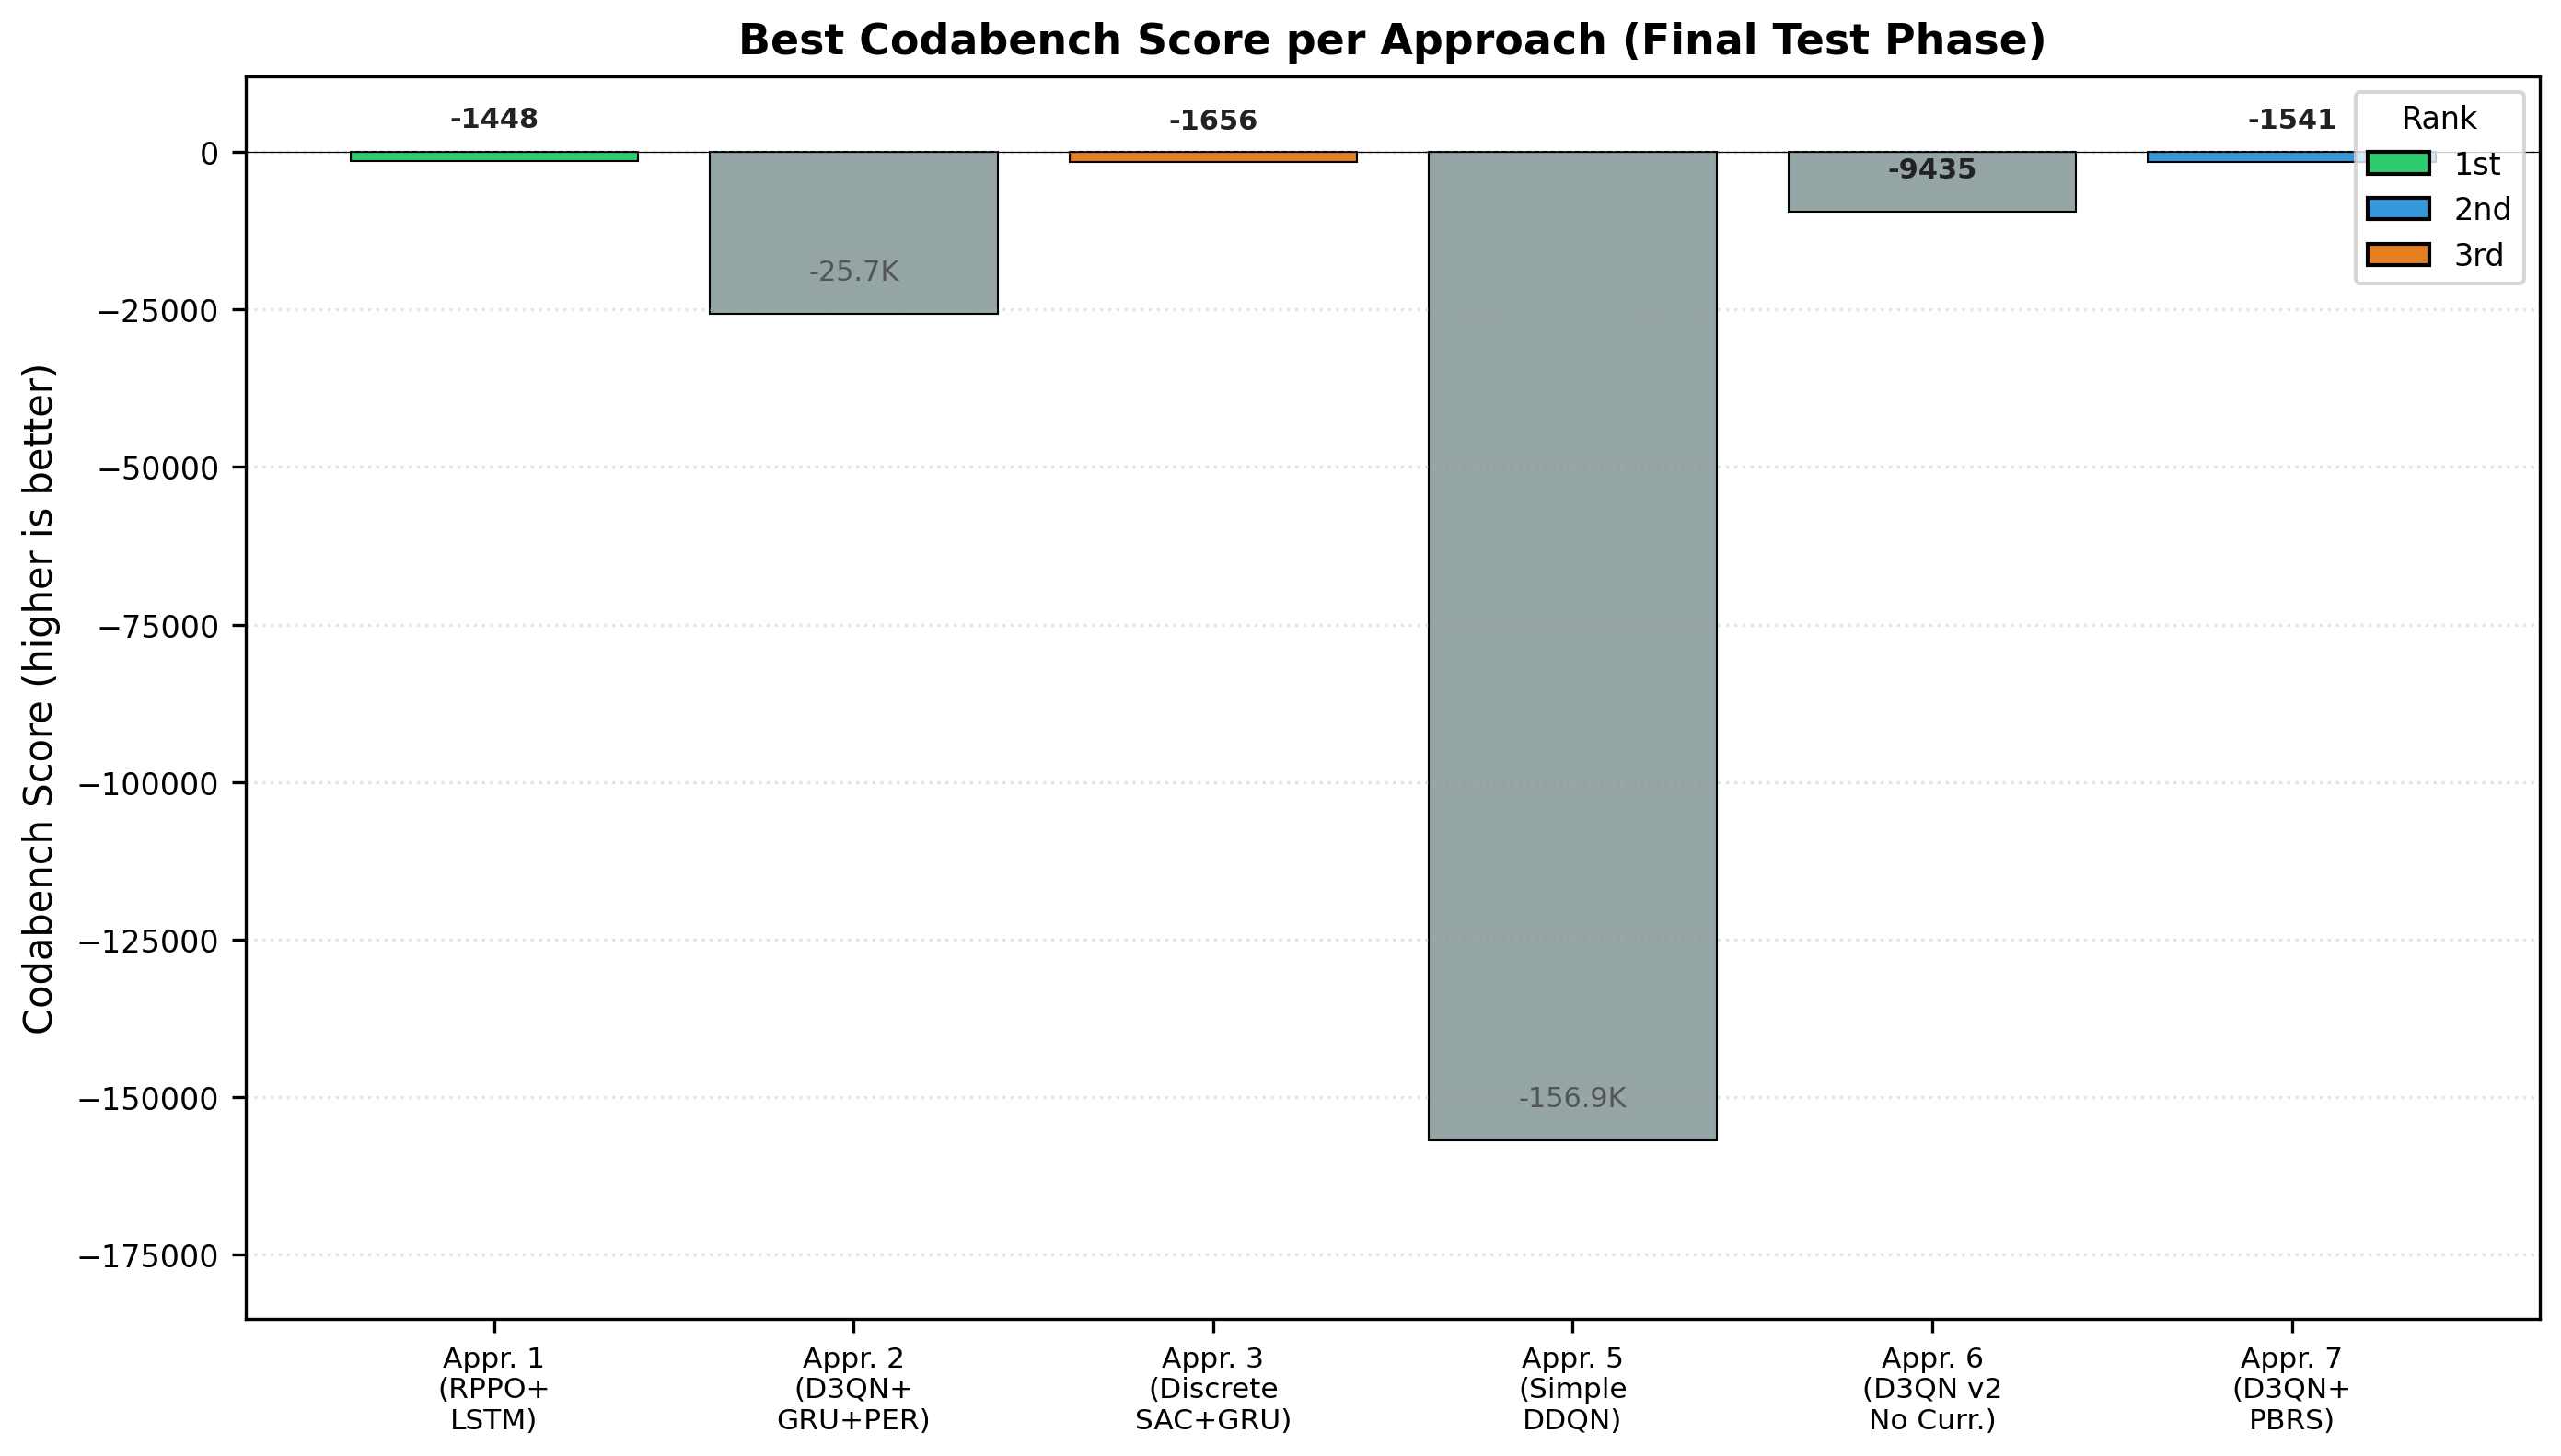
\includegraphics[width=0.6\textwidth]{16_best_score_per_approach.png}
\caption{Best Codabench score per approach on the final test phase. Approaches 1 (RPPO+LSTM) and 7 (D3QN+PBRS) significantly outperformed all others. Approach 4 (Hybrid) was not submitted to this phase.}
\label{fig:best_scores}
\end{figure}

\begin{figure}[H]
\centering
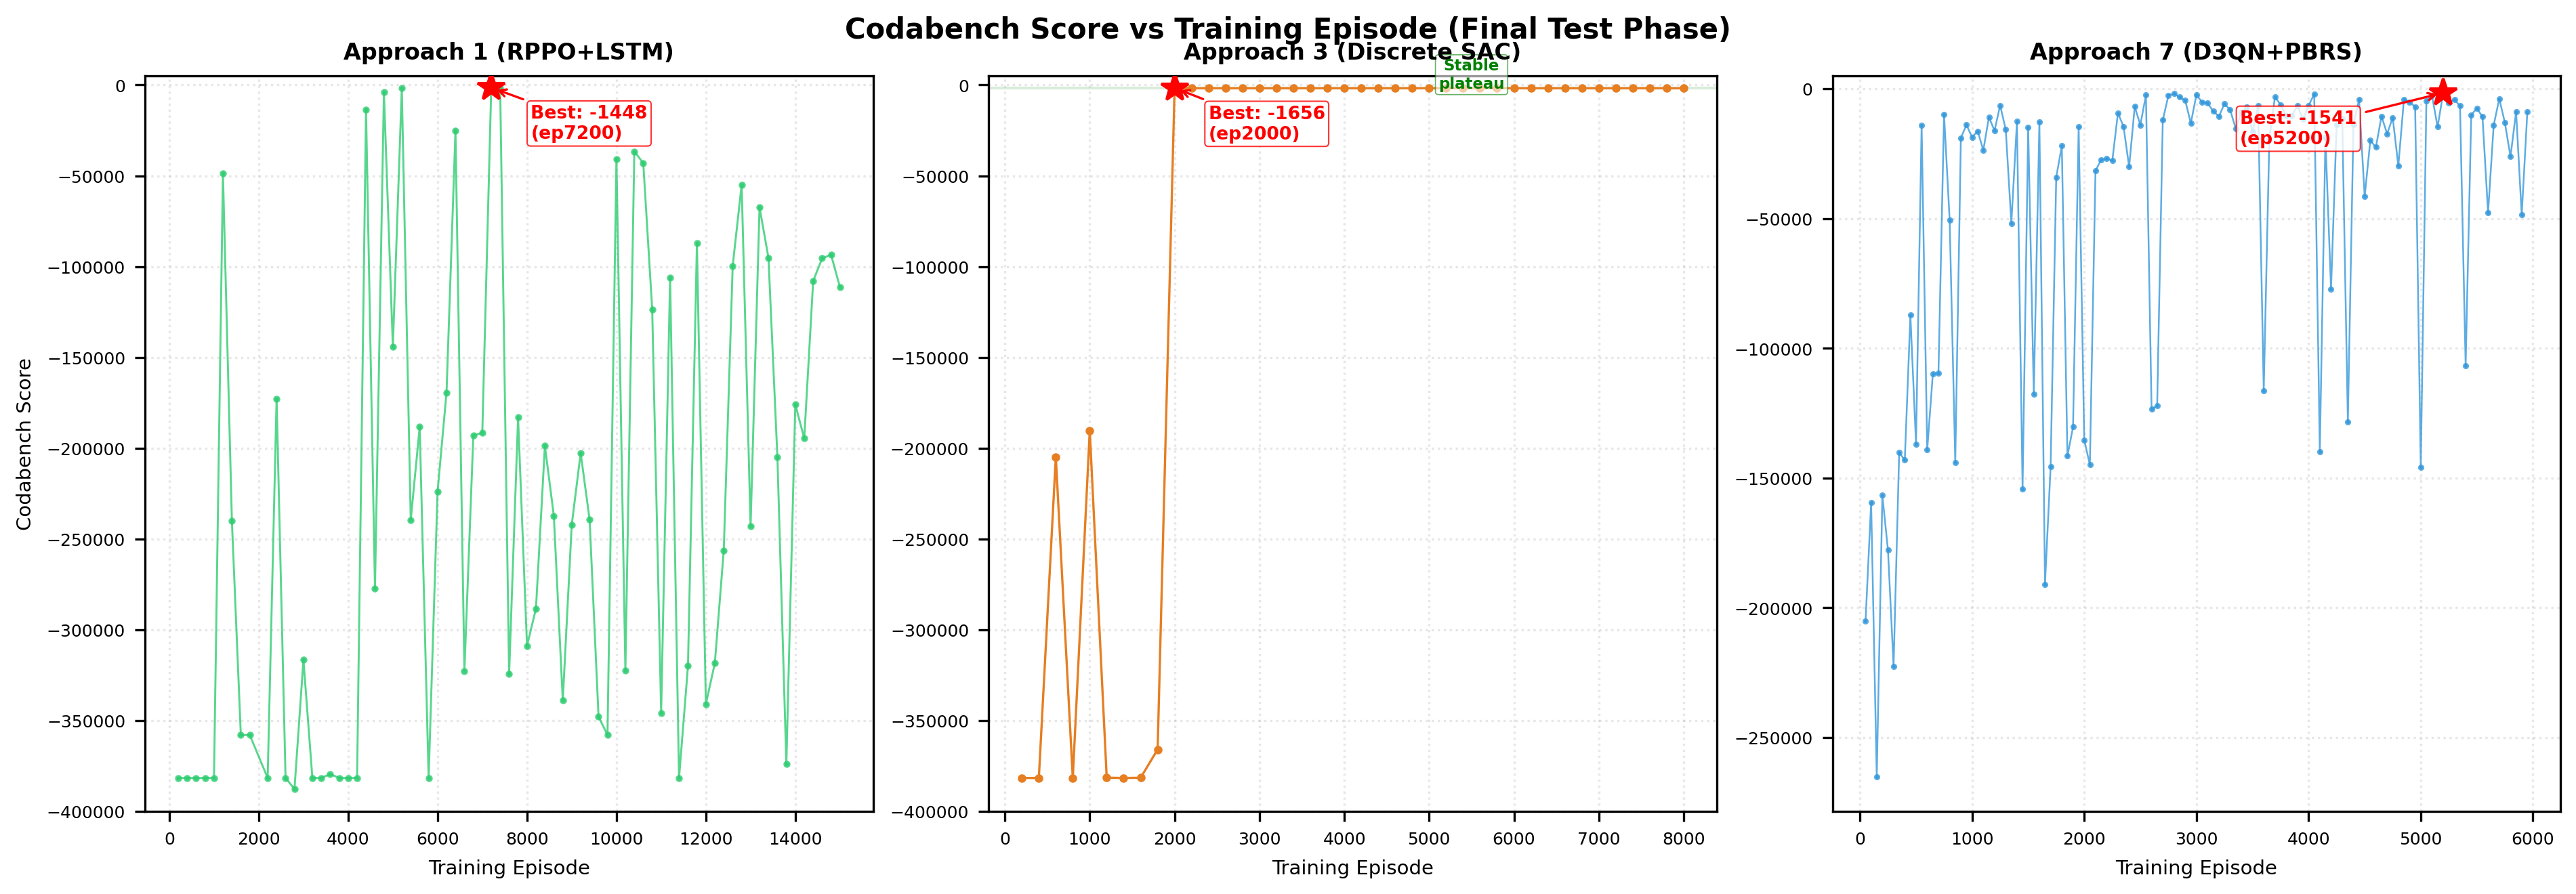
\includegraphics[width=0.75\textwidth]{17_score_vs_episode.png}
\caption{Codabench score as a function of training episode checkpoint for the three top-performing approaches. Approach 1 (RPPO) shows extreme sensitivity to checkpoint selection, Approach 3 (Discrete SAC) converges to a stable plateau after ep2000, and Approach 7 (D3QN+PBRS) exhibits high variance throughout training.}
\label{fig:score_vs_episode}
\end{figure}

\begin{figure}[H]
\centering
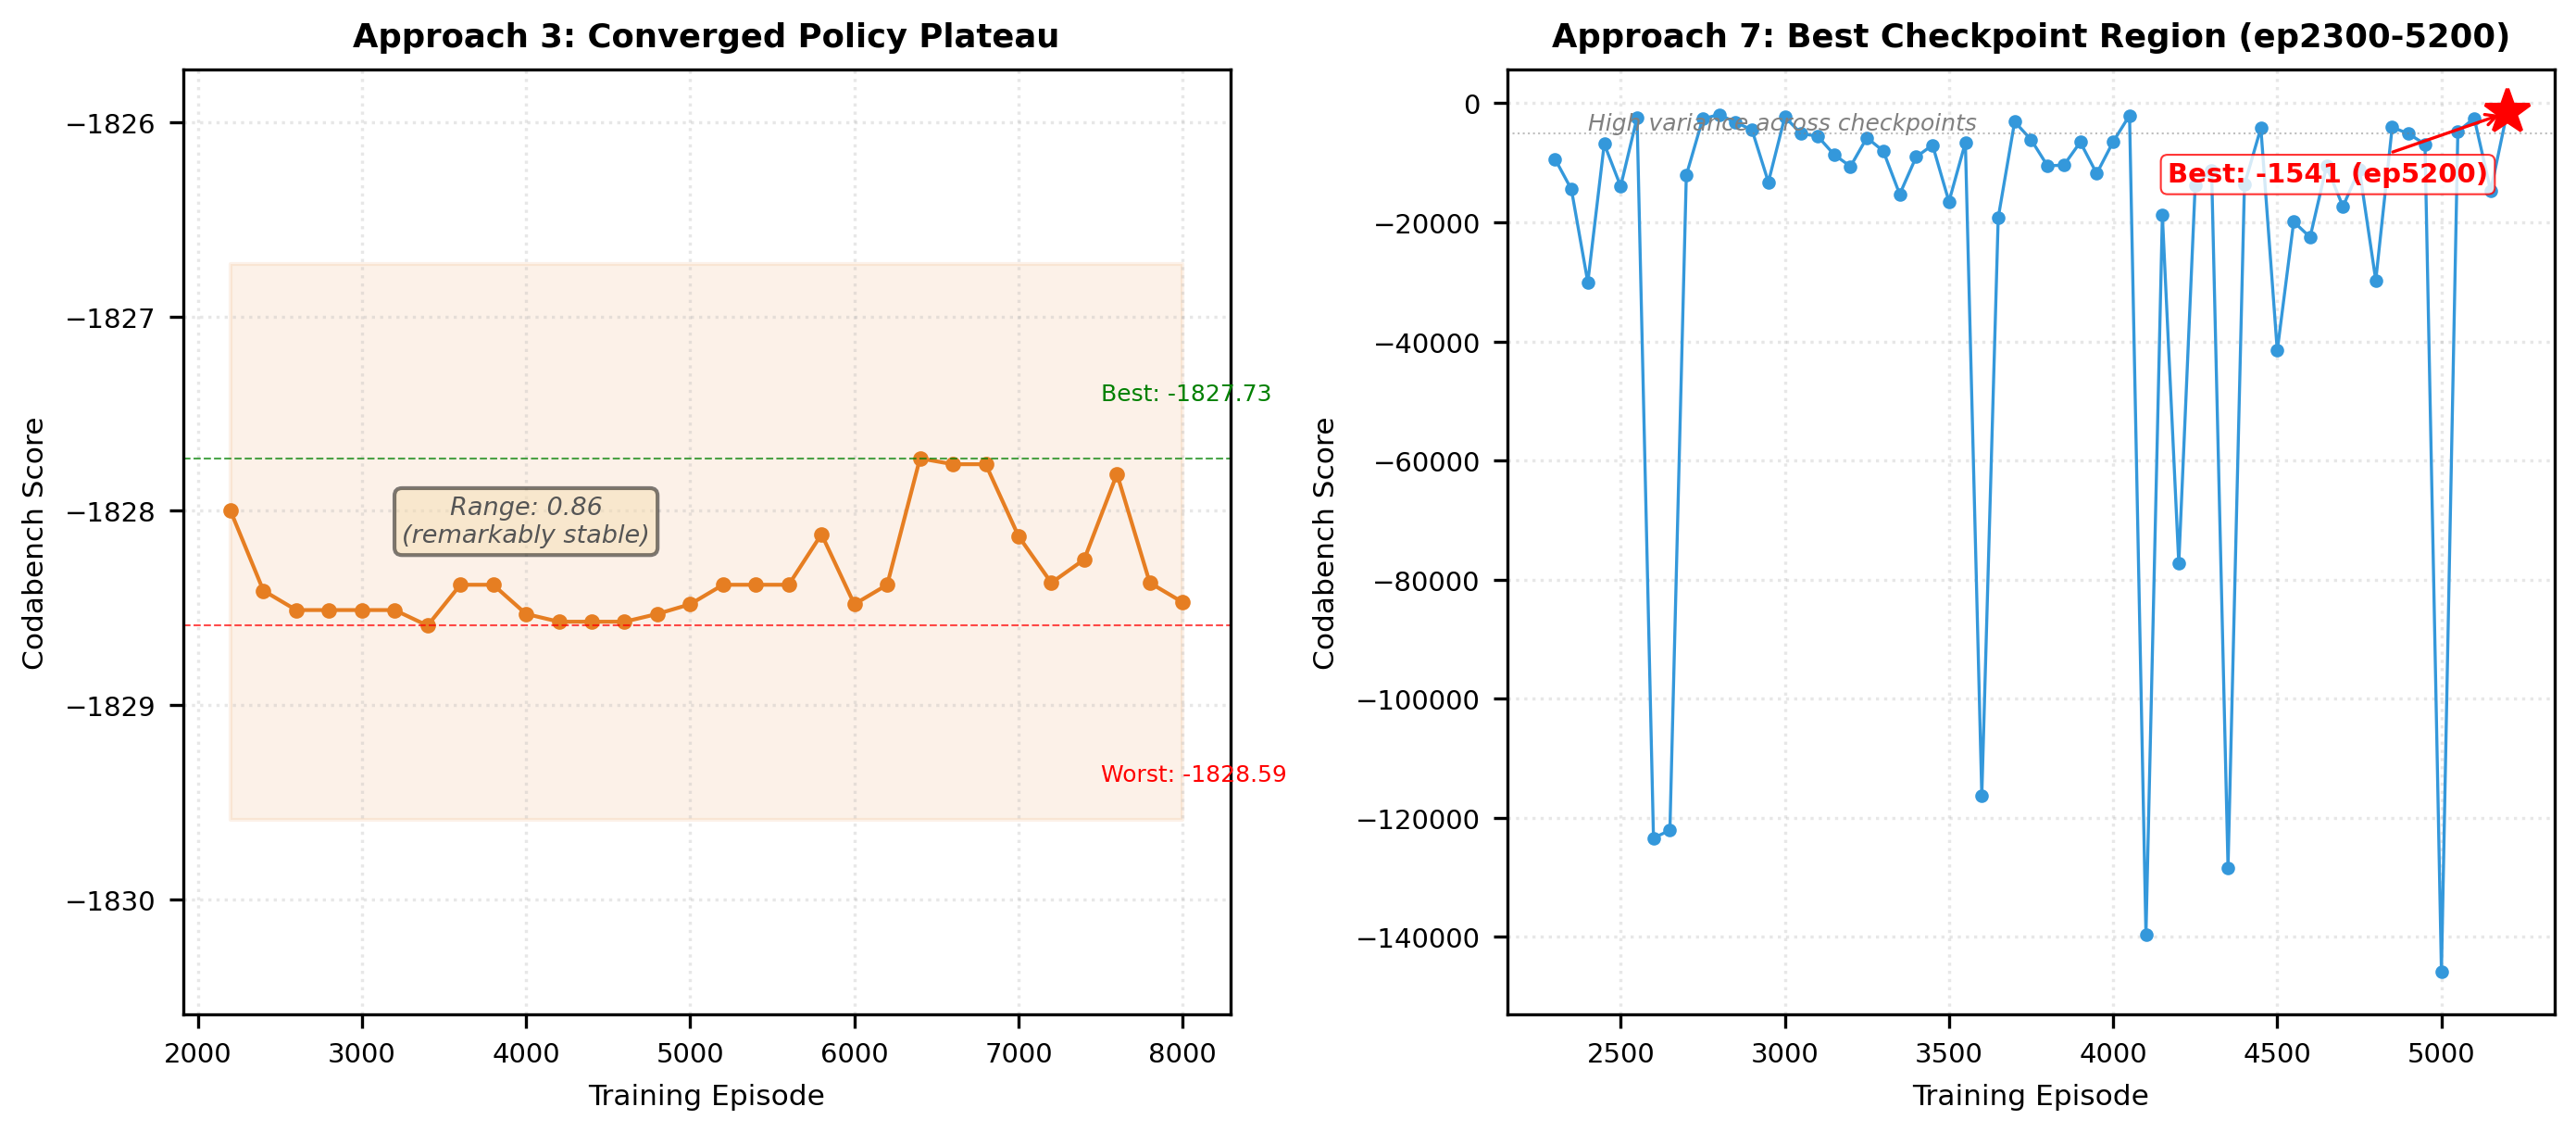
\includegraphics[width=0.77\textwidth]{18_zoomed_analysis.png}
\caption{Zoomed analysis: (Left) Approach 3's converged plateau (ep2200+) spans only $\sim$0.86 points ($-1827.73$ to $-1828.59$), indicating a stable but suboptimal local minimum. (Right) Approach 7's best region (ep2300--5200) shows extreme variance, with the best checkpoint at ep5200 ($-1541$) surrounded by checkpoints scoring $10\times$--$100\times$ worse.}
\label{fig:zoomed}
\end{figure}

\subsection{Key Observations from Results}

\hspace{12pt} \textbf{Common behavior across all agents.} Visual inspection of rollouts showed that all approaches---including the best-scoring ones---default to repetitive rotation when no sensors are active. A pure rotation policy scores roughly $-1980$ (idle penalty over 2000 steps). The score differences between approaches ($-1447$ to $-1980$) come from how well each agent responds \textit{when sensors do activate} on seeds where the box happens to spawn nearby. On most seeds, every agent rotates for the full episode.

\noindent \textbf{Method-level observations:}
\begin{itemize}[nosep]
    \item \textbf{Approach 1 (RPPO + LSTM, $-1447$)}: Best overall. The LSTM retains temporal context, and PPO's entropy regularization keeps the policy from collapsing too early. On favorable seeds it approaches, attaches, and pushes reliably. \textit{Weakness}: still rotates when sensors are zero; highly sensitive to checkpoint selection (ep7200 scores $-1447$, ep15000 scores much worse due to overfitting).
    \item \textbf{Approach 7 (D3QN + PBRS, $-1541$)}: Second best. PBRS gives a principled shaping signal and curriculum builds solid approach/push behavior. \textit{Weakness}: extreme variance across checkpoints ($-1541$ to $-156668$)---most checkpoints are bad, only a few happen to work.
    \item \textbf{Approach 3 (Discrete SAC, $-1656$ to $-1829$)}: Most stable---nearly all checkpoints from ep2200 onward score within a $\sim$0.86-point range. Entropy regularization prevents total collapse. \textit{Weakness}: converges to a fixed local optimum; the sensor-response behavior is weaker than Approaches 1 and 7, so it gains less from favorable seeds.
    \item \textbf{Approach 2 (D3QN + GRU + PER, $-25715$)}: This model had useful components (memory, prioritized replay, and n-step returns), and I trained it again in Phase 4 with sufficient compute, but it still did not work well. After many repeated all-zero observations, the GRU state became less useful, and the value updates could not recover a reliable policy for reacting to sensor signals. \textit{Strength}: it reached the best single-episode score in Phase 3 ($-1515$), but that did not become stable performance on Codabench.
    \item \textbf{Approach 6 (D3QN v2, no curriculum, $-9435$)}: Without curriculum, it never got enough near-box experience to learn approach/push behavior. GRU hidden state reset helped avoid saturation but was not enough. \textit{Strength}: simpler setup, no curriculum dependency.
    \item \textbf{Approach 5 (DDQN + heuristic, $-156899$)}: The lawnmower heuristic was a good idea for search but did not work well in practice with walls. The MLP had no recurrence, so it could not maintain temporal context. Only one submission was made.
\end{itemize}

\textbf{Curriculum learning improved sensor-conditioned control, but not box search under zero information.} Approaches 1 and 7 (with curriculum) scored $-1447$ and $-1541$, while Approaches 5 and 6 (without curriculum) scored $-156899$ and $-9435$. The main benefit of curriculum was it repeatedly exposed the agent to near-box states, so it learned better \textit{approach/attach/push} behavior once sensors became active. However, it did not solve the harder \textit{search} problem: when all sensor bits are zero, the policy still has no directional signal and often falls back to rotation. Phase 3's weaker results ($-1500$ to $-4000$) were mainly due to under-training (max\_steps$\,{=}\,$1000, stopped at $\sim$2K episodes), not a flaw in curriculum itself---Phase 4's longer training improved this.


\subsection{Learning Dynamics}

Best checkpoints appeared around episodes 5000--8000. Early episodes are too random, and later episodes tend to overfit to curriculum or shaped rewards. Approach 1's ep7200 outperformed ep15000, confirming that more training is not always better.

\section{Error Analysis and Discussion}

\subsection{Common Failure Modes}

The main failure is that when all 18 sensor bits are zero (box out of range), no approach learned to move toward the box---they all rotate in place. This means the task splits into two parts: (1) \textbf{search} (finding the box with no sensor information), which no method solved, and (2) \textbf{exploit} (acting on sensor signals once the box is detected), which curriculum-trained methods handled well.

Per difficulty level: \textbf{Level 1} fails when the box is far away (agent never detects it). \textbf{Level 2} adds blinking, so the agent can lose the signal mid-approach and revert to rotation. \textbf{Level 3} adds box movement, making accidental detection even rarer. \textbf{Walls} add $-200$ collision penalties on top of the idle penalty.

\subsection{Why Score Differences Exist}

All agents share the same rotation behavior, but scores differ because: (1) curriculum-trained agents (1, 7) respond better when sensors activate, gaining more reward from favorable seeds; and (2) the 30-seed average is sensitive to a few good seeds---one successful push episode can improve the mean by hundreds of points.

\subsection{Limitations and Future Improvements}

The biggest unsolved problem is \textit{search}: when all 18 sensor bits are zero, the agent has no information about where the box is, so it just rotates in place. None of the seven approaches solved this. Due to limited time, I could not explore the following directions, but they are promising for future work:

\begin{itemize}[nosep]
    \item \textbf{Intrinsic motivation} \cite{pathak2017curiosity, burda2018exploration}: Right now the agent only gets reward when it interacts with the box. With curiosity-based bonuses (like ICM or RND), the agent would also get a small reward for visiting new positions it has not seen before. This would push it to move around the arena instead of staying in one spot, even when sensors show nothing.

    \item \textbf{Hierarchical RL} \cite{vezhnevets2017feudal}: Instead of one policy trying to do both search and push, we could use two separate controllers---a high-level one that decides ``search for the box'' vs.\ ``go push the box,'' and a low-level one that executes each sub-task. This way each controller can specialize in its own problem.

    \item \textbf{Imitation learning} \cite{ross2011dagger}: We could first collect demonstrations from a hand-coded or human-controlled agent that searches the arena effectively (e.g., moving in a systematic pattern). Then use behavioral cloning or DAgger to train the agent to copy this behavior before fine-tuning with RL. This gives the agent a good starting policy instead of learning from scratch.

    \item \textbf{RLHF (RL from Human Feedback)} \cite{christiano2017deep}: Instead of designing a reward function manually, a human could watch agent trajectories and label which ones show good exploration vs.\ just rotating. A reward model trained on these labels would then guide the agent toward exploration behavior that is hard to specify with a simple formula.

    \item \textbf{Systematic search patterns}: The simplest solution to this problem---hard-code a lawnmower or spiral movement pattern for when all sensors are zero, and only switch to the learned RL policy when sensors activate. This is not learned behavior, but it directly solves the ``no information means no movement'' problem.

    \item \textbf{Richer observations}: The current 18-bit binary observation is very limited---either a sensor fires or it does not. Continuous sensors (e.g., distance and angle to the box) would give the agent a gradient signal even when the box is far away. Adding positional history would also help the agent remember where it has already been, so it avoids revisiting the same spots.

    \item \textbf{Domain randomization} \cite{tobin2017domain}: Training with randomized arena configurations (different spawn locations, wall layouts, box speeds) could make the policy more robust across different seeds and difficulty levels, reducing the high variance we observed in evaluation.
\end{itemize}

\section{Conclusion}

This project showed that the OBELIX task splits into two problems of very different difficulty: \textit{search} (finding the box) and \textit{exploit} (acting once the box is detected).

\begin{enumerate}[nosep]
    \item \textbf{Search remains unsolved}: All seven approaches default to rotation when sensors are inactive. The binary observation space gives no useful signal for directed movement.
    \item \textbf{Curriculum learning solves exploit}: With enough training (Phase 4), curriculum-based approaches (1 and 7) learned reliable approach/attach/push behavior, which is why they score better on seeds where the box spawns nearby.
    \item \textbf{Scores reflect sensor-response quality}: The difference between $-1447$ and $-1980$ comes from how well each agent uses favorable seeds and how well it pushes the box to boundary when seen, not from better search.
    \item \textbf{Checkpoint selection}: Best results come from mid-training checkpoints (ep5000--8000); later ones overfit.
\end{enumerate}
\hfill \break
The main takeaway: in this POMDP, the bottleneck is search, not exploitation. Curriculum learning with sufficient compute teaches the agent what to do once it finds the box, but finding the box in the first place remains the open challenge. If done any, future work should focus on intrinsic motivation, hierarchical RL, and richer state representations for a better search methodology.

\section*{Project Links}
\begin{itemize}[nosep]
    \item \textbf{YouTube Demo:} \url{PASTE_YOUTUBE_DEMO_LINK_HERE}
    \item \textbf{GitHub Repository:} \url{PASTE_GITHUB_REPO_LINK_HERE}
\end{itemize}


\section*{LLM Usage Declaration}
\begin{itemize}
\item Which Large Language Model (LLM) did you use to complete the competition or write the report? \\
Github Copilot was used in a limited advisory capacity.

\item In which part did you use the LLM, and how did it help you?

\begin{tabular}{l|l|l}
\toprule
Part & Used LLM? (Yes/No) & Purpose of Using LLM \\
\midrule
Understanding concepts & Yes & Clarifying PBRS theory, DRQN architecture details \\
Ideation / brainstorming & Yes & Generating list of possible approaches \\
Debugging small code snippets & No &   \\
Plotting / visualization code & No &   \\
Grammar / writing style & No & \\
Report structure / section ideas & Yes & ideas about how to organize content into required sections \\
Other (specify) & No &   \\
\bottomrule
\end{tabular}

\item Did you refer to any other sources or websites apart from the LLM and lecture slides? \\
Yes: (1) Sutton \& Barto textbook \cite{sutton2018reinforcement}, (2) Original OBELIX paper by Mahadevan \& Connell \cite{mahadevan1992automatic}, (3) Double DQN paper \cite{van2016deep}, (4) Dueling DQN paper \cite{wang2016dueling}, (5) PPO paper \cite{schulman2017proximal}, (6) PER paper \cite{schaul2015prioritized}, (7) PBRS paper by Ng et al.\ \cite{ng1999policy}, (8) DRQN paper by Hausknecht \& Stone \cite{hausknecht2015deep}.

\item Apart from any LLM usage, what was your own contribution? \\
All algorithmic implementation, training, hyperparameter tuning, debugging, and experimental evaluation were performed independently. The core contributions include: (1) implementing and training 7 distinct RL approaches from scratch using PyTorch based on lecture pseudocode and paper descriptions; (2) designing the heuristic fallback search policy (lawnmower pattern) based on manual play observations; (3) conducting systematic root cause analysis of the circling failure mode; (4) developing the multi-difficulty training strategy; (5) building automated checkpoint ranking and submission pipelines; (6) all experimental analysis and conclusions drawn from the results.
\end{itemize}

\vspace{1cm}

\bibliographystyle{ieeetr}
\bibliography{references}

\end{document}
